%%%%%%%%%%%%%%%%%%%%%%%%%%%%%%%%%%%%%%%%%%%%%%%%%%%%%%%%%%%%%%%%%%%%%%%%%%%
% Trim Size : 11in x 8.5in
% Text Area : 9.6in (include Runningheads) x 7in
% ws-ijbc.tex, 24 Jan 2010
% Tex file to use with ws-ijbc.cls written in Latex2E.
% The content, structure, format and layout of this style file is the
% property of World Scientific Publishing Co. Pte. Ltd.
%%%%%%%%%%%%%%%%%%%%%%%%%%%%%%%%%%%%%%%%%%%%%%%%%%%%%%%%%%%%%%%%%%%%%%%%%%%
%

%\documentclass[draft]{ws-ijbc}
\documentclass{ws-ijbc}
\usepackage{ws-rotating}     % used only when sideways tables/figures are used
\usepackage{epstopdf}
\usepackage{mathrsfs}
\usepackage{graphicx}
\usepackage{subfigure}
\usepackage{float}
\bibliographystyle{ws-ijbc}
\newcommand{\norm}[1]{\left\lVert#1\right\rVert}

\makeatletter
\newcommand*{\getlength}[1]{\strip@pt\dimexpr0.035136\dimexpr#1\relax\relax}
\newcommand{\showfont}{%
encoding: \f@encoding{},\\
family: \f@family{},\\
series: \f@series{},\\
shape: \f@shape{},\\
size: \f@size{} pt,\\
text height: \getlength{\the\textheight} cm,\\
text width:     \getlength{\the\textwidth} cm}
\makeatother


\begin{document}

\catchline{}{}{}{}{} % Publisher's Area please ignore

\markboth{Elle Musoke, Bernd Krauskopf, and Hinke M. Osinga}{A Heteroclinic Connection between Two Saddle Slow Manifolds in the Olsen Model}

\title{A Heteroclinic Connection between \\ Two Saddle Slow Manifolds in the Olsen Model}

\author{Elle Musoke, Bernd Krauskopf, and Hinke M. Osinga}


\address{Department of Mathematics, University of Auckland, Private Bag 92019\\
Auckland, 1142, New Zealand\\
elle.musoke@auckland.ac.nz}

\maketitle

\begin{history}
\received{(to be inserted by publisher)}
\end{history}

\begin{abstract}
The abstract should summarize the context, content and conclusions
of the paper. It should not contain any references or displayed
equations. Typeset the abstract in 10~pt Times Roman with
baselineskip of 12 pt, making an indentation of 1.6~cm on the left
and right margins.
\end{abstract}

\keywords{A list of 3--5 keywords are to be supplied.}
\section{Introduction}

Multiple-time scale dynamical systems are characterized by certain variables evolving on a fast time scale while other variables evolve on a slower time scale.  The separation of variables into fast and slow can be found in many systems: chemical systems, neurons, electric circuits, lasers, and predator-prey dynamics, among others, have been described by slow-fast models  \cite{BZ_reaction, Neurons, Circuits, lasers, Predator-Prey}.  In \cite{BZ_reaction}, oscillations in the Belousov-Zhabotinsky reaction are investigated.  The geometry of the oscillations arise as a consequence of a time-scale splitting in the variables.  Slow-fast models for neurons are studied in \cite{Neurons} in which excitability is the result of different time scales.  Oscillations are also studied and explained by time-scale splitting in \cite{Circuits}. A slow-fast system is used to model semi-conductor lasers in \cite{lasers}.  The role of the length of interspike intervals is investigated.  In \cite{Predator-Prey}, a slow-fast model is used to investigate the effect of a changing predator diet on predator-prey dynamics.  By reason of their ubiquity, various phenomena that arise from the multiple-time-scale nature of slow-fast systems are of significant interest. These have been described for two- and three-dimensional systems by well-established theory \cite{canard_explosion, lents-rapides, enlacement,singular_hopf, folded_node,three}.

We are concerned here with mechanisms responsible for the oscillatory behaviours exhibited by many slow-fast systems.  In two-dimensional systems canard explosions, small-amplitude limit cycles transitioning to larger-amplitude relaxation oscillations were studied, for example, in the Van der Pol oscillator and the FitzHugh--Nagumo model \cite{canard_explosion, fitz-hugh-nagumo}.  In three-dimensional systems, periodic orbits with epochs of localized small-amplitude oscillations (SAOs) and epochs of large-amplitude oscillations (LAOs) have been observed \cite{BZ}.  The mechanisms that cause SAOs of these appropriately named mixed-mode oscillations (MMOs) are described in \cite{MMO} for three-dimensional systems.  In this paper, we investigate novel phenomena that arise in four-dimensional slow-fast systems which may provide insight into undiscovered mechanisms for MMOs in higher-dimensional systems.

Previous studies exploring the mechanisms for MMOs in slow-fast dynamical systems investigate the role of so-called slow manifolds in the MMOs' generation and organisation.  Slow manifolds are families of trajectories on which the flow evolves on the slow timescale.  A slow manifold may have families of trajectories that converge toward it in forward or backward time, respectively called the stable and unstable manifolds of the slow manifold.  If a slow manifold has both a stable and an unstable manifold, it is called a saddle slow manifold.  Endocrine pituitary cells were studied with a four-dimensional slow-fast model that had a two-dimensional slow manifold in \cite{Vo_paper2}.  In \cite{Emily_Harvey_paper} a three-dimensional slow manifold was studied in a four-dimensional model for calcium oscillations inside cells. In \cite{Vo_paper} a four-dimensional model for a pituitary lactotropic cell was investigated from both a two- and three-timescale viewpoints.  From the two-timescale perspective, the model has a three-dimensional slow manifold.  In \cite{Martin_neuron_paper} a six-dimensional model for an excitable neuron was investigated.  The model had a two-dimensional slow manifold which played a role in the generation of oscillations in the system.  A five-dimensional model with a one-dimensional slow manifold was also investigated.  In \cite{Saeed_Paper} techniques were developed to compute stable and unstable manifolds of one-dimensional saddle slow manifolds in three-dimensional systems. In \cite{Cris_paper}, these techniques were generalised to compute a two-dimensional saddle slow manifold and its two-dimensional stable and unstable manifolds in the four-dimensional Hodgkin--Huxley model.  To our knowledge, there is no literature on the computation of three-dimensional (un)stable manifolds of saddle slow manifolds at this time.

We consider a prototypical four-dimensional slow-fast dynamical system that exhibits MMOs, namely an Olsen model for peroxidase-oxidase reaction.  First introduced by Lars F. Olsen in 1983  \cite{Olsen}, there are currently many different versions of the Olsen model of different dimensions.  We consider the Olsen model in the form from by \cite{Rescaling} and earlier work.  The MMO in the Olsen model phase space is of particular interest because it does not seem to be generated by the mechanisms for MMOs familiar from three-dimensional systems.

The classification of variables into those that evolve on a fast time scale and those that evolve on a slow time scale is not straightforward for the Olsen model because the variables are not consistently slow or fast over all regions of phase space.  In fact, the Olsen model nominally has three different time scales.  We focus specifically on a parameter regime corresponding to two different time scales with three fast and one slow variables.  This parameter regime was also the focus in \cite{QSSA} that reports on a study of mechanisms for MMOs after a model reduction to a three-dimensional system.  Two saddle slow manifolds were computed along with their stable and unstable manifolds.  These gave insight into the formation of the Olsen model MMO, as well as the cause of its particular geometry.  However, because of the assumptions used to reduce the model to a three-dimensional system, the dimensions of the stable manifold of one slow manifold and unstable manifold of the other were reduced to two in contrast to the corresponding three-dimensional manifolds in the full system.  

In the full system, the three-dimensional stable manifold of one slow manifold and the unstable manifold of the other are expected to intersect generically in a two-dimensional surface of connections between the two slow manifolds.  Such a surface does not generically exist in four-dimensional systems for slow manifolds of dimension larger than one.  The surface of connections also does not exist generically in systems of dimension lower than four.  In these cases, the stable and unstable manifolds of the saddle slow manifolds are limited to dimensions of two or lower and therefore do not typically have robust intersections of dimension two or higher.  In this research, we generalise the techniques in \cite{Saeed_Paper} with the aim of computing the three-dimensional stable and unstable manifolds of the one-dimensional saddle slow manifolds in the Olsen model.  Furthermore, we use our techniques in conjunction with Lin's method to compute the intersection of the three-dimensional stable and unstable manifolds in the full four-dimensional model.  This intersection is involved in the formation and organisation of an attracting MMO in our system and could lead to insights about the formation and organisation of MMOs in other higher-dimensional systems.

This paper is organized as follows.  In the next section we give the necessary background from geometric singular perturbation theory (GPST) for defining the three-dimensional manifolds which are the focus of this research.  Section 3 gives definitions of the manifolds which are then computed in section 4.  In section 5, a computation of the intersection of the manifolds computed in section 4 is described.  Conclusions are given in section 6.

%Background section
\section{The Olsen Model}

We consider the scaled system from \cite{Rescaling}, given as the system of ordinary differential equations
    
\begin{equation}
\begin{aligned}
\begin{cases}
\frac{dA}{dt} &= \mu - \alpha A - ABY, \\ \vspace{2mm}\\
\frac{dB}{dt} &= \varepsilon(1-BX - ABY), \\ \vspace{2mm}\\
\frac{dX}{dt} &= \lambda(BX - X^2 +3ABY - \zeta X + \delta), \\ \vspace{2mm}\\
\frac{dY}{dt} &= \kappa\lambda(X^2 - Y - ABY),
\end{cases}
\end{aligned}
\label{equation_1}
\end{equation}
    
\noindent
where $(A, B, X, Y)\in\mathbb{R}^{4}$ are positive concentrations of chemicals.  The system parameters are represented by the Greek letters appearing in (\ref{equation_1}) and these have the values given in Table 1.  With the minor modification, for notational convenience, of using $\varepsilon$ for $\varepsilon_{b}$ and $\frac{1}{\lambda}$ for $\varepsilon^{2}$, they are chosen to be as in \cite{Rescaling}.  The time-scaling parameters $\varepsilon$ and $\lambda$ are chosen so that we are dealing with a regime with three fast variables, $A$, $X$, and $Y$, and one slow variable, $B$.

\begin{table}[h]
\tbl{Parameters of system (\ref{equation_1}) as in \cite{Rescaling} so that $(A,X,Y)$ are fast and $(B)$ is slow.}
{\begin{tabular}{c  c  c  c  c  c  c  c  c} \\[-2pt]
\toprule
$\alpha$ & $\delta$ & $\varepsilon$ & $\lambda$ & $\kappa$ & $\mu$ & $\zeta$ \\[6pt]
\hline\\[-2pt]
0.0912 & $1.2121 \times 10^{-4}$ & 0.0037 & 18.5281 & 3.7963 & 0.9697 & 0.9847\\[1pt]
\botrule
\end{tabular}}
\end{table}
    
The classical analysis of slow-fast systems considers the two singular limits \cite{MMO}.  In the limit of $\varepsilon = 0$, system (\ref{equation_1}) reduces to
    
\begin{equation}
\begin{aligned}
\begin{cases}
\frac{dA}{dt} &= \mu - \alpha A - ABY, \\ \\
\frac{dX}{dt} &= \frac{1}{\lambda}(BX - X^2 +3ABY - \zeta X + \delta), \\ \\
\frac{dY}{dt} &= \frac{\kappa}{\lambda}(X^2 - Y - ABY),
\end{cases}
\end{aligned}
\label{equation_2}
\end{equation}
    
\noindent
with $\frac{dB}{dt}$=0, meaning that $B$ is a parameter of (\ref{equation_2}).  We refer to the three-dimensional system (\ref{equation_2}) as the fast subsystem.  Performing the time rescaling $\tau = \varepsilon t$ and then considering the limit of $\varepsilon = 0$, the system reduces to the differential algebraic reduced system
    
 \begin{equation}
\begin{aligned}
\begin{cases}
0 &= \mu - \alpha A - ABY, \\ \\
\frac{dB}{d\tau} &= (1-BX - ABY), \\ \\
0 &= \frac{1}{\lambda}(BX - X^2 +3ABY - \zeta X + \delta), \\ \\
0 &= \frac{\kappa}{\lambda}(X^2 - Y - ABY).
\end{cases}
\end{aligned}
\label{equation_3}
\end{equation}
    
\noindent
The three algebraic equations in system (\ref{equation_3}) define a one-dimensional manifold, called the critical manifold, denoted $C$.

The critical manifold $C$ consists of equilibria of the fast subsystem (\ref{equation_2}), which exist in ($A$,$B$,$X$,$Y$)-space for different values of $B$.  Their stability can be determined from the eigenvalues of the $3\times3$ Jacobian matrix of (\ref{equation_2}) evaluated at each point on the critical manifold.  Points $p \in C$ at which the Jacobian has eigenvalues with non-zero real parts are called hyperbolic.  The eigenvectors associated with the eigenvalues are categorized based on the sign of the real part of the associated eigenvalue.  Eigenvectors whose associated eigenvalues have negative real parts are called stable directions of $p$ and these span the stable eigenspace $E^{s}(p)$ of $p$.  The unstable directions and the unstable eigenspace, $E^{u}(p)$, can be defined similarly by the eigenvectors associated with eigenvalues having positive real part.  Note that the dimensions of the stable and unstable eigenspaces are equal to the number of eigenvalues with negative and positive real parts respectively.  Equilibria at which the Jacobian has eigenvalues with zero real-part are called non-hyperbolic and these correspond to bifurcations of system (\ref{equation_2}) (there are lots of introductory ODEs books, are you particular about which one I reference).

\begin{figure}[!t]
\begin{center}
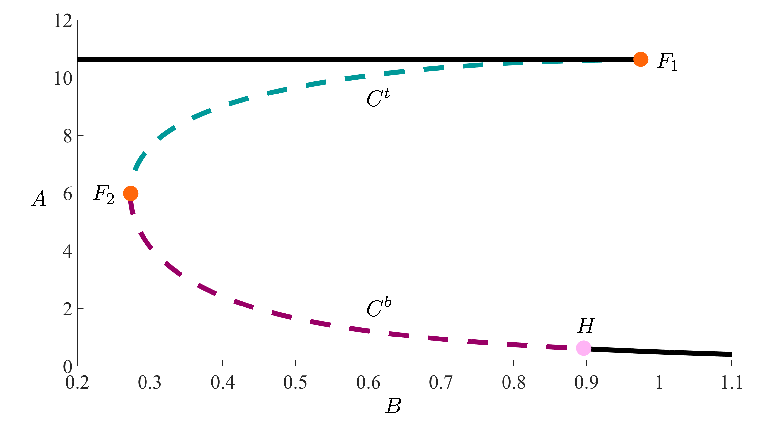
\includegraphics[page=1]{figures.pdf}
\end{center}
\caption{Physically relevant branches of the critical manifold of system (\ref{equation_1}) shown in projection onto the ($B$,$A$)-plane.  The branches labeled $C^3$ (teal) and $C^2$ (raspberry) correspond to saddle equilibria of (\ref{equation_2}), solid curves indicate stable nodes.  The two saddle-node bifurcations are represented as orange dots and labeled $F_1$ and $F_2$, respectively.  The Hopf bifurcation is labeled $H$ (pink dot).  A saddle equilibrium exists on $C^2$ and is labeled $\chi$ (green cross).}
\label{critical_figure}
\end{figure}

The critical manifold $C$ in ($A$,$B$,$X$,$Y$)-space is divided into branches by bifurcation points of the fast subsystem (\ref{equation_2}), so that points on each branch have the same dimensions of stable and unstable eigenspaces.  In other words, the branches of $C$ are one-parameter families in $B$ of hyperbolic equilibria of system (\ref{equation_2}).  In our notation for branches, superscripts indicate the dimension in ($A$,$B$,$X$,$Y$)-space of the stable eigenspace of the branch, which are defined as the collection of stable eigenspaces of all the points on the branch.  The dimension of the stable eigenspaces of the branches is, hence, one plus than the dimension of the stable eigenspace of each point on the branch.  Further, we use subscripts to distinguish the two branches on which equilibria have three-dimensional stable eigenspaces; i.e. are attracting.  

Four branches of the critical manifold lie in the physically relevant region where all phase-space variables are positive, these are shown in Figure \ref{critical_figure} projected into the ($B$,$A$)-plane.  The uppermost, black branch, denoted $C^4_+$, consists of stable equilibria of (\ref{equation_2}).  It is separated from the teal-colored branch of saddle equilibria, denoted $C^3$, by a very sharp fold point $F_1$ at $B \approx 0.956$ (orange dot).  Folds in the critical manifold correspond to saddle-node bifurcations of system (\ref{equation_2}) with respect to the parameter $B$, these are points at which one of the real eigenvalues of the Jacobian evaluated at the point switches signs.  Another fold at $B \approx 0.273$ denoted $F_2$ (orange dot), separates $C^3$ from a lower raspberry-colored branch of saddle equilibria, denoted $C^2$.   The branch $C^2$ ends at a Hopf bifurcation $H$ (pink dot) at $B \approx 0.897$.  For a Hopf bifurcation two complex-conjugate eigenvalues of the Jacobian pass through the imaginary axis of the complex plane.  To the right of $H$, there is again a stable branch of equilibria denoted $C^4_-$,.  

The point on $C^2$ at $B \approx 0.323$ is an equilibrium of system (\ref{equation_3}) and is hence an equilibrium for the full system (\ref{equation_1}).  We denote this equilibrium by $\chi$.  To the right of $W^u(\chi)$ in the $(B,A)$-projection, the flow is from right to left near $C^2$ in the full system (\ref{equation_1}).  To the left of $W^u(\chi)$ the flow is from left to right near $C^2$.  The equilibrium $\chi$ has two-dimensional stable and unstable manifolds that are denoted $W^s(\chi)$ and $W^u(\chi)$ respectively.  The manifolds $W^{s}(\chi)$ and $W^{u}(\chi)$ can be computed with conventional methods \cite{Red_book}.

Our interest is in the branches $C^3$ and $C^2$ because they are crucial for organising the phase space and are saddle objects of different type.  The branches $C^3$ and $C^2$ of the critical manifold are invariant for $\varepsilon = 0$, but not for $\varepsilon > 0$.  However, they do persist as locally invariant manifolds called slow manifolds \cite{Fenichel}.  The associated slow manifolds are traditionally denoted by $S^3_\varepsilon$ and $S^2_\varepsilon$ but, for notational convenience, we drop the subscript indicating dependence on $\varepsilon$ and refer to the slow manifolds for $\varepsilon > 0$ simply as $S^3$ and $S^2$.  The slow manifold $S^3$ has the same dimension and stability and lies at an $O(\varepsilon)$ Hausdorff distance from $C^3$.  In particular, $S^3$ converges to $C^3$ as $\varepsilon \rightarrow 0$.  For a definition of Hausdorff distance, see \cite{Hausdorff_Distance}.  Orbit segments that lie on a slow manifold remain slow for an $O(1)$ time with respect to the slow time scale.  Any trajectory that remains slow for an $O(1)$ amount of slow time can be considered to be a slow manifold.  Due to this finite time nature, slow manifolds are not unique; however any two slow manifolds lie exponentially close to each other in a suitable, $\varepsilon$-dependent neighbourhood of $C$.  A unique slow manifold, $S^2$, associated with the critical manifold branch $C^2$ can be similarly defined and selected.  To select a unique representative $S^3$ and $S^2$, we consider the slow manifold that remains slow for the longest amount of time.

The stable manifold theorem tells us that for $\frac{dB}{dt} = 0$, each $p \in C^3$ has a stable and an unstable manifold that are tangent to and have the same dimensions as $E^{s}(p)$ and $E^{u}(p)$, respectively.  We denote the stable manifold of a point $p \in C^3$ by $W^{s}(p)$ and its unstable manifold by $W^{u}(p)$.  The manifolds $W^{s}(p)$ and $W^{u}(p)$ consist of trajectories in ($A$,$B$,$X$,$Y$)-space that converge to $p$ in forward and backward time respectively.  We can then define the collection of stable manifolds for $p \in C^3$ by $W^{s}(C^3) = \bigcup_{p \in C^3} W^{s}(p)$ which is three dimensional.  We can similarly define the three-dimensional $W^{u}(C^2)$ .

According to Fenichel Theory, for $\varepsilon > 0$, $W^{s}(C^3)$ also persists in an $O(\varepsilon)$ neighbourhood as the three-dimensional local stable manifold $W^{s}_{loc}(S^3)$ of $S^3$.  The local stable manifold $W^{s}_{loc}(S^3)$ consists of families of trajectories that have a fast approach to $S^3$ then remain close to $S^3$ for $O(1)$ slow time.  The three-dimensional unstable manifold $W^{u}(S^2)$ associated with $S^2$ is similarly defined for backwards time.  Again, due to the finite-time nature of the definitions for the three-dimensional manifolds $W^{s}(S^3)$ and $W^{u}(S^2)$, they are not unique.  To select unique representatives, we consider two-parameter families of orbit segments that remain slow for the longest amount of time subject to boundary conditions described in further sections.  
 
 %Saddle slow manifold section   
 \section{Computation of saddle slow manifolds and their (un)stable manifolds}
    
The definition of a one-dimensional saddle slow manifold and its (un)stable manifolds are given in \cite{Saeed_Paper} which presents algorithms for their computation in a three-dimensional system.  We are going to define only the slow manifold $S^3$ associated with $C^3$; the slow manifold $S^2$ can be defined in a similar manner.

\subsection{Definition of $S^3$}    
The precise definition of the slow manifold $S^3$ is given with respect to a closed interval $[B_{\mathrm{in}},B_{\mathrm{out}}]$ for the slow variable $B$.  The values for $B_{\mathrm{in}}$ and $B_{\mathrm{out}}$ are chosen such that the interval is contained in the interval defined by the $B$-coordinates of the two fold points $F_1$ and $F_2$.  Note that there is a segment in $C^3$ for which each point $p \in C^3$ is uniquely associated via its $B$-coordinate with a value $B_p \in [B_{\mathrm{in}},B_{\mathrm{out}}]$.  Hence, for each $B_p \in [B_{\mathrm{in}},B_{\mathrm{out}}]$ there is a unique point $p=(p_A,p_B,p_X,p_Y) \in C^3$ such that $p_B = B_p$.  In the three-dimensional subsection $\{ \begin{pmatrix} A & B & X & Y \end{pmatrix} \in \mathbb{R}^4 \; | \; B=p_B\}$ we define a solid three-sphere $D_\delta(B_p)$ with radius $\delta$ and centre $p$ , given formally by

\begin{equation*}
D_\delta(B_p)=\{w \in \mathbb{R}^4 \; | \; w_B = B_p, \left\lVert w-p \right\rVert \leq \delta\}.
\end{equation*}
    
\noindent
The union 

\begin{equation*}
\mathscr{D} = \cup_{B_p \in [B_{\mathrm{in}}, B_{\mathrm{out}}]} D_\delta(B_p) 
\end{equation*}

\noindent
forms a four-dimensional compact cylinder.  The radius $\delta$ is small, but it needs to be at least of $O(\varepsilon)$ to ensure that $S^3$ lies in $\mathscr{D}$.  The one-parameter family of orbit segments that enter $\mathscr{D}$ via $D_\delta(B_{\mathrm{in}})$ and exit via $D_\delta(B_{\mathrm{out}})$ are candidates for $S^3$.   To select a unique representative $S^3$ that $S^3$ have maximal integration time in $\mathscr{D}$ while satisfying appropriate boundary conditions.  Our choice of boundary conditions is explained in section 3.2.
    
Figure \ref{tube_figure} shows a sketch of the unique representative, $S^3$ in green, in projection onto the $(B,A)$-plane.  Sketched in purple is $\mathscr{D}$ with the spheres $D_\delta(B_{\mathrm{in}})$ and $D_\delta(B_{\mathrm{out}})$ represented as disks at either end; these spheres and $\mathscr{D}$ are for illustration.

\begin{figure}[!t]
\begin{center}
\includegraphics[page=2]{figures.pdf}
\end{center}
\caption{The unique representative slow manifold $S^3$ (green curve) projected into the $(B,A)$-plane.  The spheres $D_\delta(B_{\mathrm{in}})$ and $D_\delta(B_{\mathrm{out}})$ are indicated by purple disks at either end of a four-dimensional cylinder, indicated by the purple curves.}
\label{tube_figure}
\end{figure}

\subsection{Definition of $W^{s}(S^3)$ and computation of $W^{s}(S^3)$ and  $S^3$}

We define $W^{s}(S^3)$ to be a two-parameter family of orbit segments that enter into $\mathscr{D}$ at $D_{\delta}(B_p)$ for some $B_p \in [B_{\text{in}}, B_{\text{out}}]$, and remain inside $\mathscr{D}$ for $O(1)$ slow time.  We select and approximate a specific candidate for $W^{s}(S^3)$ by requiring that each orbit segment lying on $W^{s}(S^3)$ have maximal integration time inside $\mathscr{D}$ while satisfying the boundary conditions explained in the following paragraphs.  We now turn to the computation of the three-dimensional manifold $W^{s}(S^3)$ in the same region the two-dimensional stable manifold was investigated in the three-dimensional reduced model considered in \cite{QSSA}.
     
As $W^{s}(S^3)$ is three dimensional it is challenging to compute and difficult to visualise.  Examples of computing and visualising three-dimensional manifolds are in \cite{Initial_conditions_volume, Invariant_tori_again, Invariant_tori}.  None of these examples are in the context of computing (un)stable manifolds of saddle slow manifolds.  Tools to implement the computation of three-dimensional manifolds are not widely used and, once computed, it is difficult to see the dynamics on the manifold in  dimensional projections.  Due to the nature of the current computation tools available, computing the entire three-dimensional manifold would also be computationally expensive compared to the the computation of two-dimensional manifolds.  A natural way forward is to consider a subset of $W^{s}(S^3)$ as a one-parameter family of two-dimensional submanifolds.  These can be computed by generalizing a method outlined in \cite{Saeed_Paper} which can then be implemented in the two-point boundary value problem (2PBVP) continuation package \textsc{Auto} \cite{AUTO}.  We begin by defining a two-dimensional plane $\Sigma$  that is transverse to the flow and $\bigcup_{p \in C^3} E^u(p)$ in our region of interest, given by fixed values of $A$ and either $X$ or $Y$.  We approximate a submanifold with a smooth, one-parameter family of solutions to (\ref{equation_1}) with the property that they begin in $\Sigma$, enter $\mathscr{D}$ at $D_{\delta}(B_p)$ for some $B_p \in [B_{\text{in}}, B_{\text{out}}]$, and remain inside $\mathscr{D}$ for $O(1)$ slow time.  We use $W^{s}_{\Sigma}$ to denote the collection of those parts of the orbit segments that enter $\mathscr{D}$ in the fast direction.  The later parts that evolve mostly in the $B$-direction inside $\mathscr{D}$ for $O(1)$ slow time are considered to approximate parts of $S^3$.  If the later part of the orbit segment includes a fast exit from $\mathscr{D}$, that fast part is considered as an approximation of an orbit segment lying on the unstable manifold of $S^3$, $W^{u}(S^3)$.

We explain first how to compute a specific submanifold $W^s_{\widehat{\Sigma}}$ for the plane $\widehat{\Sigma}$.  The plane $\widehat{\Sigma}$ is defined by the constant values $A \approx 10.6055$ and $Y \approx 0.000230006$.  These values are, respectively, the $A$- and $Y$-coordinates of the point $p_{\text{out}} \in C^3$ that has a $B$-coordinate value of $B_{\text{out}}=0.9$.  We then explain how to adjust the computation of $W^{s}_{\widehat{\Sigma}}$ for the computation of $W^{s}_\Sigma$ for a different plane, $\Sigma$.

\begin{figure}[h]
\centering
\subfigure[]{\label{step1}\includegraphics[width=8cm, height=4cm, page=3]{figures.pdf}}
\subfigure[]{\label{step2}\includegraphics[width=8cm, height=4cm, page=4]{figures.pdf}}
\subfigure[]{\label{step3}\includegraphics[width=8cm, height=4cm, page=5]{figures.pdf}}
\subfigure[]{\label{step4}\includegraphics[width=8cm, height=4cm, page=6]{figures.pdf}}
\caption{Numerical set-up for the computation of submanifolds $W^s_{\Sigma}$ of $W^s(S^3)$.  Panel (a) shows a sketch of the first homotopy step in the algorithm for computing $W^{s}_{\widehat{\Sigma}}$.  The slow manifold $S^3$ is sketched in green.  The plane $\widehat{\Sigma}$ is given by the $A$- and $Y$-coordinates of the point $p_{\text{out}}$ and is represented as a mocha line in the $(B, A)$-plane.  The linear stable space $E^s(p_{\mathrm{out}})$ is represented by a blue cross. The saddle equilibrium, $\chi$, of the full system is represented by a green x.  Panel (b) shows a representative orbit segment (purple) in the first homotopy step; fast segments are represented with double arrows while slow segments are represented with single arrows.  Panel (c) shows a sketch illustrating the selection of an orbit segment (purple) with maximal integration time that ends on the blue cube $\Omega$ spanned by the two stable eigenvectors of $p_{\text{out}}$ and the vector parallel to the $B$-direction; the one-dimensional subset $\psi$ of $\widehat{\Sigma}$ is given by fixing $B = B_{\text{in}}$ and represented in mocha.  Panel (d) shows a sketch of the selection of a different submanifold $W^{s}_{\Sigma}$ for $\Sigma$ on the other side of the critical manifold from $\widehat{\Sigma}$ with respect to the $A$-coordinate.}
\end{figure}


We compute the submanifold $W^s_{\widehat{\Sigma}}$ as a one-parameter family of orbit segments $\mathbf{u} = \{\mathbf{u}(s)| 0 \leq s \leq 1 \}$ of the rescaled system

\begin{equation}
\frac{d\mathbf{u}}{ds} = TF(\mathbf{u}),
\label{equation_4}
\end{equation}
    
\noindent
where $\mathbf{u}(s) = (A(s), B(s), X(s), Y(s)) \in \mathbb{R}^4$ is the vector of chemical concentrations, $F$ is the right-hand side of (\ref{equation_1}) and $T$ is the total integration time on the fast timescale, $t=Ts$.
    
We obtain a first solution on $W^s_{\widehat{\Sigma}}$ via a homotopy step.  Following the definition for $W^s_{\widehat{\Sigma}}$, we impose the condition
    
\begin{equation}
\mathbf{u}(0) \in \widehat{\Sigma}
\label{BC6}
\end{equation}
    
 \noindent
that is, we impose two restrictions on the startpoint of the orbit segment $\mathbf{u}$, $\mathbf{u}(0)$ because $\widehat{\Sigma}$ is two dimensional.  As part of selecting a $\mathbf{u}$ that has a fast approach and remains close to $S^3$ for $O(1)$ slow time, we consider the two-dimensional eigenspace $E^s(p^t_{\text{out}})$ that is transverse to $W^u(S^3)$.  We define the boundary condition
    
\begin{equation}
\mathbf{u}(1) \in E^s(p^t_{\text{out}})
\label{BC7}
\end{equation}
    
\noindent
that imposes two restrictions on the endpoint of $\mathbf{u}$, $\mathbf{u}(1)$ and allows for the possibility of $\mathbf{u}(1)$ intersecting $W^u(S^3)$.  The point $p_{\text{out}}$ is then a solution of the 2PBVP defined by (\ref{equation_4}), (\ref{BC6}) and (\ref{BC7}) with $T=0$.  Figure \ref{step1} illustrates the set up for this homotopy step in projection onto the $(B,A)$-plane.  Here, the plane $\widehat{\Sigma}$ is projected to a line (mocha), $E^s(p^t_{\mathrm{out}})$ is represented by a blue cross, and a line representing $S^3$ is sketched in green.  Note that in the ($B$,$A$)-projection, $\widehat{\Sigma}$ is directly underneath $C^4_+$ with respect to the variable $A$.  The saddle equilibrium $\chi$ is represented as a green x.
    
We increase the total integration time while allowing the $B$-coordinate value of $\mathbf{u}(0)$ to decrease towards $F_2$.  Note that increasing integration time in this fashion causes $T$ to become negative.  This step is illustrated in Figure \ref{step2} where an intermediate orbit segment is represented as a magenta curve illustrating the presence of a fast segment (double arrows) followed by a slow segment (single arrow).  The continuation is stopped at $\mathbf{u}(0)_B = B_{\text{in}}=0.275$, just before $\mathbf{u}(0)_B$ reaches the $B$-coordinate value of $F_2$.  A sketch of the resulting orbit segment is shown in Figure \ref{step3}.
    
The orbit segment illustrated in Figure \ref{step3} belongs to a two-parameter family of solutions $\mathbf{u}$ of (\ref{equation_4}) that satisfy the boundary conditions (\ref{BC6}) and (\ref{BC7}).  To select a one-parameter family of orbit segments from these, we select for each $B \in [B_{\text{in}}, B_{\text{out}}]$ the solution $\mathbf{u}$ with maximal integration time such that $\mathbf{u}(0)_B=B$.  To find an initial orbit segment satisfying this condition, we define the curve $\psi = \widehat{\Sigma}\cap \{ \omega \in \mathbb{R}^4 \; | \; \omega_B = B_{\text{in}}\}$ and require
    
    
\begin{equation}
\mathbf{u}(0) \in \psi,
\label{BCSTOP}
\end{equation}
    
\noindent
which imposes three conditions on $\mathbf{u}(0)$ and is more restrictive than (\ref{BC6}).  The boundary condition (\ref{BCSTOP}) is represented as a mocha line in Figure \ref{step3}.  We lessen the restrictions on $\mathbf{u}(1)$ and define the three-dimensional space $\Omega$ spanned by the two stable eigenvectors of $p_{\text{out}}$ and $\begin{pmatrix} 0, & 1, & 0, & 0 \end{pmatrix}^{tr}$.  Note that $\Omega$ is transverse to $\cup_{p \in C^3}E^u(p)$ and, hence, $W^u(S^3)$.  Instead of (\ref{BC7}) we require
    
\begin{equation}
\mathbf{u}(1) \in \Omega,
\label{BC11}
\end{equation}
    
\noindent
which imposes only one condition on $\mathbf{u}(0)$.  Condition (\ref{BC11}) is represented in Figure \ref{step3} as a cube with dark blue edges.  We now track the solution $\mathbf{u}$ of the 2PBVP (\ref{equation_4}), (\ref{BCSTOP}), (\ref{BC11}) as $T$ becomes more negative, forcing $\mathbf{u}(0)$ to approach $W^s(S^3) \cap \widehat{\Sigma}$ and $\mathbf{u}(1)$ to approach $W^u(S^3) \cap \Omega$. When a fold in $T$ is reached, a (local) minimum in the total integration time $T$ is attained.  

\begin{figure}[H]
\centering
\subfigure[]{\label{piece_BAX}\includegraphics[width=\textwidth, height=0.42\textheight, page=7]{figures.pdf}}
\subfigure[]{\label{piece_BAY}\includegraphics[width=\textwidth, height=0.42\textheight, page=8]{figures.pdf}}
\caption{The submanifold $W^{s}_{\widehat{\Sigma}}$(light blue), defined as the family of orbit segments with maximal integration time that solve the 2PBVP (\ref{equation_4}), (\ref{BCSTOP}), (\ref{BC11}) as $B$ varies.  Shown are projections into $(B,A,X)$-space (a) and $(B,A,Y)$-space (b) with a representative orbit segment plotted in magenta.  Projections of a segment of the critical manifold are shown in turquoise and the view is rotated relative to previous figures.}
\label{piece}
\end{figure}

\begin{figure}[H]
\centering
\subfigure[]{\label{two_pieces_BAX}\includegraphics[width=\textwidth, height=0.42\textheight, page=17]{figures.pdf}}
\subfigure[]{\label{two_pieces_BAY}\includegraphics[width=\textwidth, height=0.42\textheight, page=18]{figures.pdf}}
\caption{The submanifolds $W^{s}_{\Sigma}$ and $W^{s}_{\widehat{\Sigma}}$ (blue and light blue) of $W^s(S^3)$, defined as the family orbit segments with maximum integration time that solve the 2PBVP (\ref{equation_4}), (\ref{BCSTOP}), (\ref{BC11}) as $B$ varies.  Here $\Sigma$ is a plane defined by the constant values $A=2.0$ and $Y=0.0$.  Shown are projections into $(B,A,X)$-space (a) and $(B,A,Y)$-space (b) with representative orbit segments plotted in magenta on each slice.  The planes $\widehat{\Sigma}$ and $\Sigma$ are plotted in plum.  Note that $\widehat{\Sigma}$ and $\Sigma$ appear as black lines in (b) and $\widehat{\Sigma}$ is so near to $C^4_+$ that it is indistinguishable from it.  A representative illustration of the three-dimensional $\Omega$ is sketched as a blue cube.  Projections of the critical manifold are shown in black, turquoise, and raspberry and the view is rotated relative to previous figures.}
\label{two_pieces}
\end{figure}

\begin{figure}[H]
\centering
\subfigure[]{\label{pieces_BAX}\includegraphics[width=\textwidth, height=0.42\textheight, page=9]{figures.pdf}}
\subfigure[]{\label{pieces_BAY}\includegraphics[width=\textwidth, height=0.42\textheight, page=10]{figures.pdf}}
\caption{The submanifold $W^{s}_{\widehat{\Sigma}}$ and a selection of four additional $W^{s}_{\Sigma}$ (blues), defined as the family orbit segments with maximum integration time that solve the 2PBVP (\ref{equation_4}), (\ref{BCSTOP}), (\ref{BC11}) as $B$ varies.  Here, the $\Sigma$ are the planes defined by the constant values $A=2.0$ and $Y=0.0$, $A=4.0$ and $Y=0.75$, $A=4.0$ and $X=0.75$, and $A=6.0$ and $X=0.5$.  Shown are projections into $(B,A,X)$-space (a) and $(B,A,Y)$-space (b) with example orbit segments plotted in magenta.  Projections of the critical manifold are shown in black, turquoise, and raspberry and the view is rotated relative to previous figures.}
\label{pieces}
\end{figure}

    
The orbit segment that is obtained is not represented in a figure because it is almost identical to the orbit segment illustrated in Figure 3(c): it begins in $\widehat{\Sigma}$ and has a fast approach to $S^3$ before remaining $O(\varepsilon)$ close for $O(1)$ slow time, and so it lies on $W^{s}_{\widehat{\Sigma}}$ by definition.  In addition to finding an orbit segment that approximates a solution to (\ref{equation_4}) laying on $W^s_{\widehat{\Sigma}}$, we can approximate $S^3$ by restricting the orbit segment further inside $[B_{\text{in}},B_{\text{out}}]$ to exclude fast segments. At this stage the entire solution family lying on $W^s_{\widehat{\Sigma}}$ can be computed by continuing the fold in $T$, while allowing $u(0)_B$ to increase.
   
Figure \ref{piece} shows two projections of $W^s_{\widehat{\Sigma}}$.  Although the manifold is two dimensional, it is necessary to visualise it in both $(B,A,X)$- and $(B,A,Y)$-projections because it exists in four-dimensional space.  Lying on $W^s_{\widehat{\Sigma}}$ is a representative orbit segment, plotted in magenta.  The critical manifold is plotted and the view is rotated relative to earlier figures to help illustrate the geometry of the submanifold.  Orbits lying on $W^s_{\widehat{\Sigma}}$ have a fast approach to $S^3$ in $X$ and $Y$ before approaching mainly in the $A$-direction and then finally remaining close to $C^3$ for $O(1)$ slow time.
    
In the case where we would like to compute $W^{s}_{\Sigma}$ where $\Sigma$ is defined by different constant values of $A$ and $Y$ (or $X$), we can obtain a first orbit segment on $W^{s}_{\Sigma}$ via a second homotopy step.  Using an intermediate orbit segment from the first homotopy step as a starting point, we impose (\ref{BC7}) while keeping as free parameters $T$, $\mathbf{u}(0)_B$, and the $X$-coordinate $\mathbf{u}(0)_X$ of $\mathbf{u}(0)$ (or the $Y$-coordinate  $\mathbf{u}(0)_Y$ of $\mathbf{u}(0)$).  In two runs, we continue $\mathbf{u}$ with $\mathbf{u}(0)_A$ and $\mathbf{u}(0)_Y$ (or $\mathbf{u}(0)_X$) as main continuation parameters.  In each of these runs, we increase or decrease the main continuation parameter until it attains the value necessary for $\mathbf{u}(0) \in \Sigma$.  Once $\mathbf{u}(0) \in \Sigma$, we follow the rest of the procedure described above while considering $\Sigma$ instead of $\widehat{\Sigma}$.
    
Figure \ref{step4} illustrates a choice of $\Sigma$ on the opposite side of the critical manifold from $\widehat{\Sigma}$ with respect to the $A$-coordinate in the ($B$,$A$)-projection.  The orbit segment resulting from the second homotopy step is represented as a magenta curve.  Conditions (\ref{BCSTOP}) and (\ref{BC11}) are again illustrated with a mocha line and a cube with dark blue edges, respectively.

Figure \ref{two_pieces} shows $W^s_{\widehat{\Sigma}}$ together with one other submanifold $W^{s}_{\Sigma}$ of $W^{s}(S^3)$.  The additional submanifold was selected with $\Sigma$ given by $A=2.0$ and $Y=0.0$.  Figure \ref{pieces} shows the two submanifolds of $W^{s}$ shown in Figure \ref{two_pieces} along with three additional submanifolds and the planes $\Sigma$ that define them.  The additional submanifolds were selected with $\Sigma$ given by $A=4.0$ and $X=0.75$, $A=4.0$ and $Y=0.75$, and $A=6.0$ and $X=0.5$.  Note that the $\Sigma$ appear as lines in one of the two projections, depending on whether they are defined by constant values of $X$ or $Y$.  The submanifolds appear to intersect, however this is due to the variable $A$ being slower than variables $X$ and $Y$.  This causes orbit segments to approach $S^3$ in the $X$- and $Y$-directions before approaching in the $A$-direction and is the reason for the portions of the submanifolds that come very near to each other.
    
We note that, unlike the stable manifold of $S^3$ computed for the reduced system in \cite{QSSA}, each submanifold $W^{s}_{\Sigma}$ in Figure \ref{pieces} diverges backwards in time in the $X$- and $Y$- directions before reaching $S^2$.  The computations in \cite{QSSA} suggest that there exists a  submanifold of $W^s(S^3)$ in the four-dimensional system that spirals around $S^2$ in backward time for an appropriate choice of $\Sigma$.  Such a surface would be the intersection of the two three-dimensional manifolds $W^s(S^3)$ and $W^u(S^2)$ in the full four-dimensional system.  

%unstable
\subsection{Definition and computation of $W^{u}(S^2)$}  

Before investigating the existence of such an intersection, we first consider the unstable manifold $W^{u}(S^2)$ of $S^2$.  The computation of submanifolds of $W^{u}(S^2)$ is similar to the computation of $W^{s}_\Sigma$, however adjustments must be made in light of some complicating challenges.  Two extra challenges are the saddle equilibrium, $\chi$, of the full system lying on $C^2$ at $B = 0.323$ and the Hopf bifurcation of the fast subsystem at $B = 0.897$.  Additional care must be taken to ensure that the computed orbits do not increase in integration time solely by approaching the saddle equilibrium's stable manifold or by following the nearby stable slow manifold backward in time.  Values for $B_{\mathrm{in}}$ and $B_{\mathrm{out}}$ are chosen such that $\chi_B < B_{\mathrm{out}} < B_{\mathrm{in}}< H_B$.  We can then define the four-dimensional cylinder $\mathscr{D}$ similarly to how it was defined for $W^s(S^3)$.  The unstable manifold can then be defined as a two-parameter family of orbit segments composed of a collection of one-parameter families that enter $\mathscr{D}$ at $B_{\mathrm{in}}$, follow $S^2$ for an $O(1)$ amount of slow time and then exit at $B_p$ for each $B_p \in [B_{\mathrm{in}}, B_{\mathrm{out}}]$.  We modify the steps for computing two-dimensional submanifolds of $W^s(S^3)$ in order to ensure that an increase in integration time results only from a more accurate approximation of a submanifold of $W^u(S^2)$.

Namely, we must make adjustments to boundary conditions so that orbit segments do not increase in integration time by approaching $\chi$ or by following the attracting slow manifold to the right of the Hopf bifurcation in the $(B,A)$-projection in backwards time.  To compute a submanifold of $W^u(S^2)$, we define for each $B_p \in [B_{\mathrm{in}}, B_{\mathrm{out}}]$ a sphere in the subspace $\{B=B_p\}$, centered at $p$ and with radius $r$; here $p \in C^2$ is the unique point such that $p_B = B_p$.  More formally,

\begin{equation*}
\widetilde{D}_r(B_p)=\{w \in \mathbb{R}^4 \;|\; w_B = B_p, \left\lVert w-p \right\lVert  = r\}.
\end{equation*}

\noindent
We can then define the three-dimensional cylinder $\mathscr{R} = \cup_{B \in [B_{\mathrm{in}}, B_{\mathrm{out}}]}\widetilde{D}_r(B)$.  

We define a submanifold $W^u_r$ for $r>\delta$, as the one-parameter family of orbit segments that enter $\mathscr{D}$ at $B_{\mathrm{in}}$ and, for each $B_p \in [B_{\mathrm{in}}, B_{\mathrm{out}}]$, intersect $\mathscr{R}$ after exiting $\mathscr{D}$ at $B_p$ an $O(1)$ amount of slow time afterwards.  The radius $\delta$ is chosen small enough so that $\mathscr{R}$ does not contain a locus of points at which the flow is not transverse to $\mathscr{R}$.  We use the cylinder $\mathscr{R}$ instead of the plane $\Sigma$ described in section 4.1 to keep the endpoints of orbit segments $\mathbf{u}$ close enough to $C^2$ so that the $\mathbf{u}$ cannot contain segments that approach $\chi$.  In the following steps, the computation of a submanifold $W^u_{r^*}$ is outlined for $r^*=0.7$ before the description of the necessary modifications to obtain $W^u_r$ for more general $r$. 

We perform an initial homotopy step analogous to the homotopy step in section 4.1 to obtain an orbit segment that enters $\mathscr{D}$ at $B_{\mathrm{in}}$ and intersects $\mathscr{R}$ after exiting $\mathscr{D}$ at some $B^* \in [B_{\mathrm{in}}, B_{\mathrm{out}}]$.  We select the unique point $\bar{p} \in C^2$ such that $\bar{p}_B=0.7$.  The plane $\bar{\Sigma}$ is defined by fixing the $A$- and $Y$- coordinates of $\bar{p}$, which are $A \approx 0.940272$ and $Y \approx 1.342954$.  We impose the boundary conditions

\begin{equation}
\mathbf{u}(0) \in E^u(\bar{p}),
\label{BC1_unstable}
\end{equation}

\noindent
and 

\begin{equation}
\mathbf{u}(1) \in \bar{\Sigma}
\label{BC2_unstable}
\end{equation}
\noindent
which each impose two conditions on $\mathbf{u}(0)$ and $\mathbf{u}(1)$, respectively.  The point $\bar{p}$ is then a solution to the 2PBVP defined by (\ref{equation_4}), (\ref{BC1_unstable}), and (\ref{BC2_unstable}) for $T=0$.  We increase $T$ while $\mathbf{u}(1)_B$ decreases and stop the continuation when $\mathbf{u}(1)$ intersects $\mathscr{R}$.  This step is almost identical to the initial homotopy step in section 4.1 except that we reverse the direction of time and instead of stopping the continuation when $\mathbf{u}(1)_B$ attains a certain value, we stop the continuation when $u(1)$ intersects $\mathscr{R}$.  We denote by $B_{\mathrm{stop}}$ the $B$-value of $\mathbf{u}(1)$ at the end of this step and $p^{stop}$ the corresponding point in $C^2$.

We perform a second homotopy step to ensure that $\mathbf{u}(0)$ is such that $\mathbf{u}$ can approach $S^2$ for $O(1)$ slow time while also ensuring that $\mathbf{u}$ doesn't increase in integration time by following the attracting slow manifold for longer backward time.  In the second homotopy step we define a three-dimensional space $\Xi_{\textsc{hom2}} = E^u(\bar{p}) + span\{ \begin{pmatrix} 0 & B & 0 & 0 \end{pmatrix}^{tr} \}$ and a one-dimensional circle $\Theta = \{ w \in \mathbb{R}^4 \; | \; w_Y=\bar{p}_Y, w_B=B_{\mathrm{stop}}, \left\lVert w-p^{\mathrm{stop}} \right\lVert=0.7\}$.  Then the orbit segment resulting from the first homotopy step is a solution to the 2PBVP defined by (\ref{equation_4}),

\begin{equation}
\mathbf{u}(0) \in \Xi_{\textsc{hom2}},
\label{BC3_unstable}
\end{equation}

\noindent
and 

\begin{equation}
\mathbf{u}(1) \in \Theta.
\label{BC4_unstable}
\end{equation}
\noindent
Our goal is to continue the orbit segment by increasing $T$ such that $u(0)_B$ increases, that is (\ref{BC3_unstable}) drives the continuation.  Condition (\ref{BC4_unstable}) is chosen such that integration time does not increase with decreasing $\mathbf{u}(1)_B$ and so that our 2PBVP is well defined.  The continuation is stopped when $\mathbf{u}(0)_B =1.0$.  The resulting orbit segment is initially attracted to the attracting slow manifold and follows it until it passes near $\mathscr{H}$ at which point $\mathbf{u}$ follows $S^2$.  As following the attracting slow manifold for longer backwards time requires the increase of $\mathbf{u}(0)_B$, we fix $\mathbf{u}(1)_B$ from this step onwards to ensure that this does not occur.  This is different from section 4.1 in which $\mathbf{u}(1)_B$ remained unfixed in the final steps of the computation. 

To fix $\mathbf{u}(0)_B$, we define the plane $\Phi = \{w \in \Xi_{\textsc{hom2}} \; | \;  w_B=1.0\}$ and impose the boundary conditions

\begin{equation}
\mathbf{u}(0) \in \Phi,
\label{BC5_unstable}
\end{equation}

\noindent
and 

\begin{equation}
\mathbf{u}(1) \in \{ w \in \mathscr{R} \; | \; w_B=B_{\mathrm{stop}}\}.
\label{BC6_unstable}
\end{equation}
\noindent
Condition (\ref{BC6_unstable}) requires that $\mathbf{u}(1)$ remain on a two-dimensional sphere as opposed to the one-dimensional curve $\psi$ described for condition ($\ref{BCSTOP}$) in section 4.1.  We must allow this extra degree of freedom for $\mathbf{u}(1)$ as keeping $\mathbf{u}(0)_B$ fixed in condition $(\ref{BC5_unstable}$) imposes an extra constraint compared to condition ($\ref{BC11}$) in section 4.1.  Our aim is to select a smooth one-parameter family of orbit segments from the two-parameter family of orbit segments satisfying the 2PBVP defined by $(\ref{equation_4})$, ($\ref{BC5_unstable}$), and ($\ref{BC6_unstable}$) to which the orbit segment resulting from the second homotopy step is a solution.  To this end, for each $B_p \in [B_{\mathrm{in}},B_{\mathrm{out}}]$, we select from the one-parameter family of orbit segments exiting $\mathscr{D}$ at $B_p$ the orbit segment with maximal integration time.  To find an initial orbit of this description we increase $T$ again until maximal integration time is reached.  This is detected as a fold in $T$.  Finally to obtain the rest of the submanifold $W^u_{r^*}$ we switch the endpoint boundary condition to

\begin{equation}
\mathbf{u}(1) \in \mathscr{R}
\label{BC7_unstable}
\end{equation}
\noindent
which imposes one condition on $\mathbf{u}(1)$.  In two runs, the fold in $T$ is continued until $\mathbf{u}(0)_B=B_{\mathrm{out}}=0.35$ and then again until $\mathbf{u}(0)_B=B_{\mathrm{in}}=H_B$ to sweep out $W^u_{r^*}$.

Figure \ref{unstable_piece} shows two projections of the submanifold $W^u_{r^*}$.  Example orbit segments lying on $W^u_{r^*}$ are plotted in forest green and a subset of $C^2$ is plotted in raspberry.  The view is rotated relative to previous figures.

We can compute a different submanifold $W^u_r$ by returning to the second homotopy step in our computation.   Depending on the magnitude of $r$, we may need to perform one or two additional homotopy steps.  In the case where $r$ is large enough that $\widetilde{D}_r(\mathbf{u}(1)_B)$ contains a locus of points at which the flow is not transverse to it, an extra homotopy step is needed.  We define a plane $\Xi_{\mathrm{hom3}}$ by fixing the $A$- and $X$-coordinates of $\mathbf{u}(1)$ after the second homotopy step.  To ensure that our 2PBVP is well defined, the orbit segment is continued with the boundary conditions (\ref{BC5_unstable}) and

\begin{equation}
\mathbf{u}(1) \in \Xi_{\mathrm{hom3}},
\label{BC8_unstable}
\end{equation}
\noindent
which imposes two conditions on $\mathbf{u}(1)$.  The endpoint $B$-coordinate $\mathbf{u}(1)_B$ is increased until $\widetilde{D}_r(\mathbf{u}(1)_B)$ no longer contains a locus of tangent points.

The final homotopy step involves defining another plane $\Xi_{\mathrm{homfinal}}$ by fixing the $B$- and $X$- values of $\mathbf{u}(1)$.  Condition (\ref{BC5_unstable}) is imposed while a new restriction

\begin{equation}
\mathbf{u}(1) \in \Xi_{\mathrm{homfinal}},
\label{BC9_unstable}
\end{equation}
\noindent
imposes two conditions on $\mathbf{u}(1)$.  The radius $r$ is then increased or decreased until the desired magnitude is attained.  All that remains is to follow through with the rest of the steps to compute $W^u_r$.  In the last step, $B_{\text{out}}$ is chosen such that the flow is transverse to $\widetilde{D}(B_{\text{out}})$.We do not show several submanifolds of $W^u(S^2)$ in the same figure, because the spiralling dynamics near $C^2$ make visualisation difficult in the $(B,A,X)$- and $(B,A,Y)$-projections due to (self)-intersections of the submanifolds in these projections.

\begin{figure}[H]
\centering
\subfigure[]{\label{piece_BAX_unstable}\includegraphics[width=\textwidth, height=0.42\textheight, page=15]{figures.pdf}}
\subfigure[]{\label{piece_BAY_unstable}\includegraphics[width=\textwidth, height=0.42\textheight, page=16]{figures.pdf}}
\caption{The submanifold $W^u_{r^*}$ (red) of $W^u(S^2)$ computed as the family of orbit segments with maximal integration time that are solutions to the 2PBVP $(\ref{equation_4})$, $(\ref{BC5_unstable})$, and $(\ref{BC7_unstable})$ projected into $(B,A,X)$-space (a) and $(B,A,Y)$-space (b) with example orbit segments plotted in forest green.  Projections of a segments of the critical manifold are shown in black and raspberry and the view is rotated relative to previous figures.}
\label{unstable_piece}
\end{figure}


%Lin's method

\section{A heteroclinic connection between two saddle slow manifolds}

\begin{figure}[h]
\centering
\subfigure[]{\label{hetclin1}\includegraphics[width=8cm, height=4cm, page=11]{figures.pdf}}
\subfigure[]{\label{hetclin2}\includegraphics[width=8cm, height=4cm, page=12]{figures.pdf}}
\subfigure[]{\label{hetclin3}\includegraphics[width=8cm, height=4cm, page=13]{figures.pdf}}
\subfigure[]{\label{hetclin4}\includegraphics[width=8cm, height=4cm, page=14]{figures.pdf}}
\caption{}
\end{figure}


The two three-dimensional manifolds $W^s(S^3)$ and $W^u(S^2)$ are likely to intersect generically in a two-dimensional manifold of heteroclinic connections in the four-dimensional phase space.  We we denote the surface of intersections $\mathscr{H}$.  We can compute such a surface of connections with an approach known as Lin's method \cite{Lin_original, Lin_POs, Lin_POs2}.  Since Lin's method is typically used in parameter continunation of heteroclinic connections that are not structurally stable, we explain the set-up here for our context.  We first choose a three-dimensional so-called Lin section $\mathscr{L}$ that divides the four-dimensional phase space into two regions such that $S^3$ lies in one region and $S^2$ is in the other.  We then compute an orbit segment $\mathbf{u}$ lying on $W^s(S^3)$ and continue it in several homotopy steps until $\mathbf{u}(0) \in \mathscr{L}$.  We also compute an orbit segment $\mathbf{w}$ on $W^u(S^2)$ and continue it until  $\mathbf{w}(1) \in \mathscr{L}$ as well.

We define a vector $\mathbf{v}_Z \in \mathbb{R}^4$ called a Lin vector and given by 

	\begin{equation}
		\mathbf{v}_Z = \frac{\mathbf{u}(0) - \mathbf{w}(1)}{\left\lVert \mathbf{u}(0) - \mathbf{w}(1) \right\lVert}
		\label{Lin_vector}
	\end{equation}
	
\noindent	
as well as two unit normal vectors $\mathbf{n}_1, \mathbf{n}_2 \in \mathscr{L}$ such that $\mathbf{n}_i \perp \mathbf{v}_Z$ for $i=1,2$ and $\mathbf{n}_1 \perp \mathbf{n}_2$.  While our choice for the vector $\mathbf{v}_Z$, and normal vectors $\mathbf{n}_1$ and $\mathbf{n}_2$ is arbitrary, their selection remains fixed for the remainder of the computation.  The span of $\mathbf{v}_Z$ defines a one-dimensional space, $Z \subset \mathscr{L}$, called a Lin space.  The distance between $\mathbf{u}(0)$ and $\mathbf{w}(1)$ in $Z$ defines the a Lin gap which is a regular test function which we denote $\eta$.  We approximate an orbit segment on $\mathscr{H}$ by continuation in the direction of decreasing $\eta$ while requiring $\mathbf{u}(0), \mathbf{w}(1) \in Z$.  When  $\eta = 0$, an orbit segment on $\mathscr{H}$ is detected as the concatenation of $\mathbf{w}$ and $\mathbf{u}$ at this continuation step.

In our computations of $\mathbf{u}$ and $\mathbf{w}$ we do not find the orbit segments with maximal integration time as it is not straightforward to track two folds simultaneously with the automatic fold continuation in the package \textsc{Auto} \cite{AUTO}.  A discussion of the numerical accuracy of our results follows in the next section.  Since we are not requiring that $\mathbf{w}$ satisfy the condition of maximal integration time, we do not run into the same issues encountered in section 4.2 for the computation of a submanifold of $W^u(S^2)$.  For this reason we may compute $\mathbf{w}$ without considering the distance of $\mathbf{w}(1)$ from $C^2$.

\subsection{Computing an initial orbit segment on $W^s(S^3)$}

The Lin section $\mathscr{L}$ is a three-dimensional section given by a constant $A$-coordinate.  We choose $\mathscr{L} = \{\omega \in \mathbb{R}^4 \; | \; \omega_A = 6.0 \}$ so that, in the ($B$,$A$)-projection and with respect to the variable $A$, it lies between $\chi$ and the point on $C^3$ with the same $B$-coordinate as $\chi$.  Our choice of $\mathscr{L}$ allows us to avoid stopping the continuation because $\mathscr{L}$ has intersected $C^2$.  We can instead compute the largest possible portion of $\mathscr{H}$ by continuing orbit segments as close as possible to $\chi$.  Although $\mathscr{L}$ is three dimensional, it is illustrated as a purple line in the ($B$, $A$)-projection in Figure \ref{hetclin1}.

We compute the orbit segment $\mathbf{u}$ as in the computation of an initial orbit segment on a submanifold $W^s_{\Sigma}$ in section~3.2 with the exception that we omit last the step and do not compute the orbit with maximal integration time.  Here, $\Sigma$ is the plane given by $A=6.0$ and $Y\approx1.342954$.

\subsection{Computing an initial orbit segment on $W^u(S^2)$}

We perform three homotopy steps to obtain an initial orbit segment on $W^u(S^2)$.  We begin with the point $\bar{p}$ that is a solution to the 2PBVP defined by $(\ref{equation_4})$, (\ref{BC1_unstable}), and (\ref{BC2_unstable}) for $T=0$.  We obtain an orbit segment $\mathbf{w}$ by imposing conditions (\ref{BC1_unstable}) and (\ref{BC2_unstable}) while increasing integration time.  The continuation is stopped when $\mathbf{w}(1)_B = 0.6$.

We then impose (\ref{BC3_unstable}) and (\ref{BC2_unstable}) while additionally requiring $\mathbf{w}(1)_B=0.6$.  We continue $\mathbf{w}$ while increasing integration time once more while $\mathbf{w}(0)_B$ increases, and stop the continuation when $\mathbf{w}(0)_B=1.0$.

In the third homotopy step, we impose (\ref{BC5_unstable}) while keeping $\mathbf{w}(0)_B$, $\mathbf{w}(1)_B$ and $\mathbf{w}(1)_Y$ fixed.  The $A$-coordinate of $\mathbf{w}(1)$ increases as $T$ is increased.  The continuation is stopped when $\mathbf{w}(1)_A = 6.0$.  In other words, we stop the continuation when $\mathbf{w}(1) \in \mathscr{L}$.

\subsection{Closing the Lin gap}

We are now in a position to define vectors $\mathbf{v}_Z$, $\mathbf{n}_1$, and $\mathbf{n}_2$.  We define $\mathbf{v}_Z$ using the orbit segments $\mathbf{u}$ and $\mathbf{w}$ obtained in sections 5.1 and 5.2 and take $\mathbf{n}_1 = \begin{pmatrix} 0, & 0, & \mathbf{v}_{Z_Y}, & -\mathbf{v}_{Z_X} \end{pmatrix}^{tr}$, and $\mathbf{n}_2 = \begin{pmatrix} 0, & \mathbf{v}_{Z_Y}, & 0, & -\mathbf{v}_{Z_B} \end{pmatrix}^{tr}$.  We impose conditions

\begin{align}
	\begin{split}
		\mathbf{u}(0), \mathbf{w}(1) \in \mathscr{L},\\ \vspace{2mm}
		[\mathbf{u}(0) - \mathbf{w}(1)] \cdot \mathbf{n}_1 =0, \\ \vspace{2mm}
		[\mathbf{u}(0) - \mathbf{w}(1)] \cdot \mathbf{n}_2 =0
	\end{split}
	\label{Z}
\end{align}

\noindent
to restrict  $[\mathbf{u}(0) -\mathbf{w}(1)] \in Z$.  Additionally, we impose conditions (\ref{BC7}) and (\ref{BC5_unstable}) while allowing the integration times of $\mathbf{u}$ and $\mathbf{w}$ to move freely.  The pair of orbit segments $\mathbf{u}$ and $\mathbf{w}$ obtained at the end of section 5.2 are one of a two-parameter family of orbit-segment pairs satisfying (\ref{BC7}), (\ref{BC5_unstable}), and (\ref{Z}).  To formulate a well-defined 2PBVP, we impose the restriction

\begin{equation}
\mathbf{w}(1)_B \in \{ \omega \in \mathbb{R}^4 \; | \; \omega_B = 0.6 \},
\label{fix_B}
\end{equation}  
\noindent
and continue $\mathbf{u}$ and $\mathbf{w}$ while $\eta$ is decreased.  We stop the continuation as soon as $\eta = 0$, at which point the concatenation of $\mathbf{w}$ with $\mathbf{u}$ forms an approximation of a heteroclinic connection in $\mathscr{H}$.

To obtain a one-parameter family of concatenations approximating $\mathscr{H}$, we require $\eta = 0$ while relaxing condition (\ref{fix_B}).  We then decrease $\mathbf{w}(1)_B$ and stop the continuation before $\mathbf{u}$ and $\mathbf{w}$ reach the intersection of $\mathscr{H}$ with $W^u(\chi)$.  We sweep out the other side of the manifold by continuation in the opposite direction (of increasing $\mathbf{w}(1)_B$) and stop just before $\mathbf{w}(1)_B$ reaches the $B$-coordinate of the Hopf bifurcation point $H$ on $C^2$.

Figure \ref{heteroclinic} shows $\mathscr{H}$ projected into $(B,A,X)$- and $(B,A,Y)$-space.  The portion of $\mathscr{H}$ composed of the collection of orbit segments $\mathbf{w}$ is colored in red and the portion composed of orbit segments $\mathbf{u}$ is blue.  Orbit segments on $\mathscr{H}$ spiral around $S^2$ for an $O(1)$ amount of slow time before exiting via $W^u(S^2)$ and following $S^3$ for an $O(1)$ amount of slow time via $W^s(S^3)$.  Three representative orbit segments are shown, their $\mathbf{w}$ segments in magenta and their $\mathbf{u}$ segments in forest green.

\begin{figure}[H]
\centering
\subfigure[]{\label{hetclin_BAX}\includegraphics[width=\textwidth, height=0.42\textheight, page=21]{figures.pdf}}
\subfigure[]{\label{hetclin_BAY}\includegraphics[width=\textwidth, height=0.42\textheight, page=22]{figures.pdf}}
\caption{The heteroclinic connection $\mathscr{H}$ projected into (a) $(B,A,X)$- and (b) $(B,A,Y)$-space.  The portion of $\mathscr{H}$ that was computed as orbit segments in $W^s(S^3)$ is plotted in blue while the portion that was computed as orbit segments laying on $W^u$ associated with $S^2$ is plotted in red.  Three representative orbit segments laying on $\mathscr{H}$ are plotted.  The portions of the orbit segments computed as $\mathbf{u}$ are plotted in magenta while the segments that were computed as $\mathbf{w}$ are plotted in forest green.  The Lin section $\mathscr{L}$ is plotted in charcoal.  Although $\mathscr{L}$ appears as a plane in the two projections, it is indeed three dimensional.  The saddle equilibrium $\chi$ is plotted as a green cross, partially obstructed by $\mathscr{H}$, $\mathscr{L}$, and its unstable manifold, $W^{u}(\chi)$.  The unstable manifold $W^{u}(\chi)$ is plotted in burgundy.  The critical manifold is plotted and the view is rotated relative to previous figures to facilitate viewing.}
\label{heteroclinic}
\end{figure}


%Singular surface computation

\section{Computing the singular surface of heteroclinic connections}

The computation of the surface of heteroclinic connections, $\mathscr{H}^*$, for $\varepsilon=0$ is slightly different from the computation of $\mathscr{H}$ for $\varepsilon > 0$.  The time scaling parameter, $\varepsilon$, being zero means that $\mathscr{H}^* = W^s(C^3) \cap W^u(C^2)$.  The surface $\mathscr{H}^*$ is then composed of the family of heteroclinic connections in (\ref{equation_2}) parameterized by $B$.  In the ($B$,$A$)-projection on $C^2$, the equilibria to the left of $B \approx 0.476858$ have all real eigenvectors and equilibria to the right have a complex conjugate pair of eigenvectors.  Due to the change in the type of eigenvectors, two slightly different algorithms are used to compute $\mathscr{H}$ in two pieces.  We first describe the computation for equilibria with real eigenvectors and then for equilibria with complex conjugate eigenvectors.  

For both computations, we consider solutions to the rescaled system

\begin{equation}
\frac{d\mathbf{u}}{ds} = TG(\mathbf{u}),
\label{fast_rescale}
\end{equation}

\noindent
where $\mathbf{u}(s) = (A(s), X(s), Y(s)) \in \mathbb{R}^3$ is the vector of chemical concentrations, $G$ is the right hand side of (\ref{equation_2}), and $T$ is integration time on the fast timescale $t=Ts$.  The Lin section $\mathscr{L}$ is again taken to be the space defined by a constant $A=6.0$.  Note that in the layer equation, $\mathscr{L}$ is two dimensional and $B$ is a parameter.

\subsection{Real eigenvalues}

For the first three steps of the computation, the parameter $B$ is kept constant at a value of $0.4$.  We compute an initial orbit segment on $W^{s}(C^3)$ following the algorithm for computing a two-dimensional global manifold as a solution family of BVPs outlined in \cite{Red_book}.  We consider the equilibrium $\tilde{p}_{\Re}$ of (\ref{equation_2}) for $B=0.4$ such that $\begin{pmatrix} \tilde{p}_{\Re_A},& 0.4,&\tilde{p}_{\Re_X},&\tilde{p}_{\Re_Y} \end{pmatrix} \in C^3$.  We define a plane $\widetilde{\Sigma}_{\Re} = \{ \omega \in \mathbb{R}^3  \; | \; \omega_Y = \tilde{p}_{\Re_Y} \}$ and a one-dimensional circle $\widetilde{\Gamma}_{\Re}= \{ \omega \in \mathbb{R}^3  \; | \; \tilde{p}_{\Re} + r_{\Re}(\mathbf{v}_1\sin(\theta) + \mathbf{v}_2\cos(\theta)), \theta \in [0,2\pi) \}$  where $r_{\Re}=0.0001$ and $\mathbf{v}_1$ and $\mathbf{v}_2$ are the stable eigenvectors of $\tilde{p}_{\Re}$.  The radius $r_{\Re}$ of $\widetilde{\Gamma}_{\Re}$ is chosen small enough that $\widetilde{\Gamma}_{\Re}$ approximates a curve lying on $W^{s}(\tilde{p}_{\Re})$ and large enough that $\textsc{Auto}$ can distinguish points on $\widetilde{\Gamma}_{\Re}$ from $\tilde{p}_{\Re}$.  The point $\tilde{p}_{\Re} + r_{\Re}\mathbf{v}_2$ is then a solution to the 2PBVP defined by (\ref{fast_rescale}) and the conditions

\begin{equation}
	\mathbf{u}(1) \in \widetilde{\Gamma}_{\Re},
	\label{top_end}
\end{equation}

and

\begin{equation}
	\mathbf{u}(0) \in \widetilde{\Sigma}_{\Re}
\end{equation}

\noindent
for $T=0$.  An initial orbit segment, $\mathbf{u}$, on $W^{s}(C^3)$ with start point in $\mathscr{L}$ is obtained by decreasing $\mathbf{u}(0)_A$ while also allowing integration time to increase in backwards time, corresponding to negative $T$.  The continuation is stopped when $\mathbf{u}(0) \in \mathscr{L}$, in other words, when $\mathbf{u}(0)_A = 6.0$.

In the second step, we obtain an initial orbit segment on $W^{u}(C^2)$ with end point in $\mathscr{L}$ through almost identical means.  We consider the equilibrium $\hat{p}_{\Re}$ of (\ref{equation_2}) for $B=0.4$ such that $\begin{pmatrix} \hat{p}_{\Re_A}, &0.4, & \hat{p}_{\Re_X}, & \hat{p}_{\Re_Y} \end{pmatrix} \in C^2$ and the unstable eigenvectors $\mathbf{k}_1$ and $\mathbf{k}_2$ of $\hat{p}_{\Re}$.  We then define $\widehat{\Gamma}_{\Re} = \{ \omega \in \mathbb{R}^3  \; | \; \tilde{p}_{\Re} + r_{\Re}(\mathbf{v}_1\sin(\theta) + \mathbf{v}_2\cos(\theta)), \theta \in [0,2\pi) \}$.  The point $\hat{p}_{\Re} + r_{\Re}\mathbf{k}_2$ is then a solution to the 2PBVP defined by (\ref{fast_rescale}) and the conditions

\begin{equation}
	\mathbf{w}(0) \in \widehat{\Gamma}_{\Re}
	\label{bottom_start}
\end{equation}

and

\begin{equation}
	\mathbf{w}(1) \in \widehat{\Sigma}_{\Re},
\end{equation}

\noindent
for $T=0$.  We increase $\mathbf{w}(1)_A$ while also allowing integration time to increase in forward time, corresponding to positive $T$.  The continuation is stopped when $\mathbf{w}(1) \in \mathscr{L}$.

In the third step, we define the Lin vector 

\begin{equation}
	\mathbf{v}_Z = \frac{\mathbf{u}(0) - \mathbf{w}(1)}{\left\lVert \mathbf{u}(0) - \mathbf{w}(1) \right\lVert},
	\label{Lin_vector_singular}
\end{equation}

\noindent
that is three dimensional.  We also define a normal vector $\mathbf{n} = \begin{pmatrix} 0, & -\mathbf{v}_{Z_Y}, &-\mathbf{v}_{Z_X} \end{pmatrix}$ such that $\mathbf{n} \perp \mathbf{v}_Z$.  We then define the conditions 

\begin{align}
	\begin{split}
		\mathbf{u}(0), \mathbf{w}(1) \in \mathscr{L} \\ \vspace{2mm}
		\begin{pmatrix}\mathbf{u}(0) - \mathbf{w}(1)\end{pmatrix} \cdot \mathbf{n} =0.
	\end{split}
	\label{singular_Z}
\end{align}

\noindent
To close the Lin gap, $\eta$ we impose conditions (\ref{top_end}), (\ref{bottom_start}), and (\ref{singular_Z}) while decreasing $\eta$ and allowing integration time to move freely.  The continuation is stopped when $\eta = 0$ at which point the concatenation of $\mathbf{w}$ with $\mathbf{u}$ forms an approximation of a heteroclinic connection on $\mathscr{H}^*$.  We can then sweep out the portion of $\mathscr{H}^*$ corresponding to real eigenvalues increasing and decreasing the parameter $B$ inside the interval ($F_{2_B}$, 0.47685750162] while requiring that $\eta=0$.  We choose to stop our continuation at $B = 0.47685750162$, before the eigenvalues switch from real to complex conjugate.

\subsection{Complex conjugate eigenvalues}

The method for computing an initial orbit segment, $\mathbf{u}$, on $W^{s}(C^3)$ for complex conjugate eigenvalues is similar except that throughout the computation and the definitions of associated surfaces, we substitute $\tilde{p}_{\Re}$ for the equilibrium $\tilde{p}_{\Im}$ of \ref{equation_2} for $B=0.7$ such that $\begin{pmatrix}\tilde{p}_{\Im_A}, &0.7, &\tilde{p}_{\Im_X}, &\tilde{p}_{\Im_Y} \end{pmatrix}$.

The computation of orbit segments on $W^u(C^2)$ for $B$-values whose corresponding equilibria on $C^2$ that have complex conjugate eigenvalues presents the additional challenge.  Namely, some orbit segments on $W^u(C^2)$ contain a segment that spirals tightly around $C^2$ while others do not.  Orbit segments that spiral require larger mesh sizes than those that do not, however mesh size is held constant in our continuation.  To address this issue, we define a radius $r_{\Im} =  f(B)$, where $f(B)$ is the linear function such that $f(0.47685750164)=0.0001$ and $f(0.86)=0.2$.  This allows us to avoid the tightly spiralling regions by choosing a start point farther away from $C^2$ in those areas.

To compute an initial orbit segment, $\mathbf{w}$, on $W^u(C^2)$, we begin by considering the equilibrium $\hat{p}_{\Im}$ of (\ref{equation_2}) for $B=0.7$ such that $\begin{pmatrix} \hat{p}_{\Im_A},& 0.7,&\hat{p}_{\Im_X},&\hat{p}_{\Im_Y} \end{pmatrix} \in C^2$.  $\widehat{\Sigma}_{\Im} = \{ \omega \in \mathbb{R}^3  \; | \; \omega_Y = \hat{p}_{\Im_Y} \}$ and a one-dimensional circle $\widehat{\Gamma}_{\Re}= \{ \omega \in \mathbb{R}^3  \; | \; \hat{p}_{\Im} + f(0.7)(\mathbf{h}_1\sin(\theta) + \mathbf{h}_2\cos(\theta)), \theta \in [0,2\pi) \}$  where $\mathbf{h}_1$ and $\mathbf{h}_2$ are the real and complex parts of the unstable complex conjugate eigenvectors of $\hat{p}_{\Re}$.  The point $\hat{p}_{\Im} + f(0.7)\mathbf{h}_2$ then becomes a solution to the 2PBVP defined by (\ref{fast_rescale}) and the conditions

\begin{equation}
	\mathbf{w}(0) \in \widehat{\Gamma}_{\Im}
	\label{bottom_start_complex}
\end{equation}

and

\begin{equation}
	\mathbf{w}(1) \in \widehat{\Sigma}_{\Im},
\end{equation}

\noindent
for $T=0$.  To obtain a $\mathbf{w}$ such that $\mathbf{w}(1) \in \mathscr{L}$, we increase $\mathbf{w}(1)_A$ while allowing $T$ to increase and stop the continuation when $\mathbf{w}(1)_A=6.0$.

We close the Lin gap by imposing the conditions (\ref{top_end}), (\ref{Lin_vector_singular}), and (\ref{bottom_start_complex}) while decreasing $\eta$ and allowing integration to move freely.  The continuation is stopped when $\eta=0$ at which point the concatenation of $\mathbf{w}$ with $\mathbf{u}$ forms an approximation of a heteroclinic connection on $\mathscr{H}^*$.  We can then sweep out the portion of the manifold corresponding to complex conjugate eigenvalues by increasing and decreasing the parameter B inside the interval $[0.47685750164, H)$ while requiring that $\eta=0$.  We choose to stop the continuation at $B=0.47685750164$ before the eigenvalues switch from complex conjugate to real.

%\subsection{Complex eigenvalues}
%
%We compute an initial orbit segment, $\mathbf{w}$, on $W^{u}(C^2)$ by imposing
%
%We consider the equilibrium $\tilde{p} \in C^2$ and define a one-dimensional circle $\Gamma = \{ \omega \in \mathbb{R}^3  \; | \; \tilde{p} + r(\mathbf{v}_1\sin(\theta) + \mathbf{v}_2\cos(\theta)), \theta \in [0,2\pi) \}$ where $r=0.0001$ and $\mathbf{v}_1$ and $\mathbf{v}_2$ are respectively the real and imaginary parts of the complex conjugate eigenvectors of $\tilde{p}$.  We also define the plane $\widetilde{\Sigma} = \{ \omega \in \mathbb{R}^3 \; | \;  \omega_B = \tilde{p}_Y \}$.  The point $\tilde{p} + r\mathbf{v}_2$ is then a solution to the 2PBVP defined by (\ref{equation_4}) and the conditions.  
%
%\begin{equation}
%	\mathbf{u}(0) \in \Gamma,
%\end{equation}
%
%and
%
%\begin{equation}
%	\mathbf{u}(1) \in \widetilde{\Sigma}
%\end{equation}
%
%\noindent
%for $T=0$.  The radius $r$ is chosen small enough that it approximates a point on $W^{u}(\tilde{p})$ and large enough that $\textsc{Auto}$ can distinguish $\tilde{p} + r\mathbf{v}_2$ from $\tilde{p}$.  It is important that $r$ be chosen large enough, otherwise the arclength of $\mathbf{u}$ will not increase in the second step of the continuation.  An initial orbit segment on $W^{u}(C^2)$ is obtained by increasing $\mathbf{u}(1)_A$ while also allowing $T$ to increase.  The continuation is stopped when $\mathbf{u}(1) \in \mathscr{L}$, in other words, when $\mathbf{u}(1)_A = 6.0$.

\bibliography{elle}

\end{document}

%%------------------------------------------------------------------------------------------------------------------------------------------------------------------------------------------------------------------------------------------------------------------------------------------------------------------------------------------------------------------------------------------------------------------------------------------------------------------------

%                                                                                                                                                                                                   SECTION GRAVEYARD: RESURRECTIONS AVAILABLE UPON REQUEST
%

%------------------------------------------------------------------------------------------------------------------------------------------------------------------------------------------------------------------------------------------------------------------------------------------------------------------------------------------------------------------------------------------------------------------------------------------------------------------------

%%---------------------------------------------------------------------------------------------------------------------------------------------------------------------
%                                                                         2PBVP SET-UP FOR S^3
%%---------------------------------------------------------------------------------------------------------------------------------------------------------------------


%\subsection{Boundary value implementation}
%    
%We compute $S^3$ by setting up an appropriately defined two-point boundary-value problem (2PBVP) with the pseudo-arclength continuation package \textsc{Auto} \cite{AUTO}.  We view $S^3$ as an orbit segment $\mathbf{u} = \{\mathbf{u}(s)| 0 \leq s \leq 1 \}$ of the rescaled system
%
%
%\begin{equation}
%\frac{d\mathbf{u}}{ds} = TF(\mathbf{u}),
%\label{equation_4}
%\end{equation}
%    
%\noindent
%where $\mathbf{u}(s) = (A(s), B(s), X(s), Y(s)) \in \mathbb{R}^4$ is the vector of chemical concentrations, $F$ is the right-hand side of (\ref{equation_1}) and $T$ is the total integration time on the fast timescale, $t=Ts$.
%    
%To obtain an initial solution of (\ref{equation_4}), we perform a homotopy step as follows.  First, we choose $B_{\mathrm{out}} = 0.75$ at a value that corresponds to a point $p_{\mathrm{out}} \in C^3$ close to $F_1$.  We then impose the conditions
%    
%\begin{equation}
%\mathbf{u}(0) \in \cup_{p \in C^3} E^u(p),
%\label{BC3}
%\end{equation}
%and
%\begin{equation}
%\mathbf{u}(1) \in E^s(p^t_{\mathrm{out}}),
%\label{BC2}
%\end{equation}
%\noindent
%that each impose two conditions on $\mathbf{u}(0)$ and $\mathbf{u}(1)$, respectively.  The point $p$ is then a solution to the two-point boundary-value problem defined by (\ref{equation_4})--(\ref{BC2}) with $T=0$.  We then  decrease $\mathbf{u}_B(0)$ towards $F_2$ while the total integration time increases.  The integration is stopped when $\mathbf{u}_B(0)=B_{\text{in}}=0.4$, corresponding to a point $p_{\text{out}} \in C^3$, before it reaches $F_2$.
%    
%We remark that $D_\delta(B_{\mathrm{in}})$ defines a three-parameter family of orbit segments with initial conditions in the sphere.  We can refine our search for orbits that enter the cylinder via $D_\delta(B_{\mathrm{in}})$ and exit it via $D_\delta(B_{\mathrm{out}})$ by observing that, because $S^3$ is of saddle type, the initial point of a candidate orbit segment must lie in a small neighborhood of $W^s$ in the sphere $D_\delta(B_{\mathrm{in}})$.  Similarly the end point must remain in a small neighborhood of $W^u$ in the sphere $D_\delta(B_{\mathrm{out}})$.
%    
%We define the two-dimensional plane $\Phi = \{E^u(p^t_{\mathrm{in}}) + \begin{pmatrix} 0 & 0 & 0 & B \end{pmatrix}^{tr}| B \in \mathbb{R} \}$ that is transverse to $W^s \cap D_{\delta}(B_{\mathrm{in}})$ and contains $E^u(p_{\text{stop}})$.  We impose the boundary conditions
%    
%\begin{equation}
%\mathbf{u}(0) \in \Phi
%\label{BC1}
%\end{equation}
%    
%\noindent
%which impose two conditions on $\mathbf{u}(0)$.  The orbit segment resulting from the homotopy step is then a solution to the 2PBVP defined by (\ref{equation_4}), (\ref{BC2}), and (\ref{BC1}).  The total integration time $T$ is a free parameter in this 2PBVP, which means that there exists a one-parameter family of solutions.  To select a unique orbit segment from this solution family, we impose the additional condition that $T$ be locally maximal.  This will be the orbit segment which locally has the longest slow segment in the geometric sense and will be the best approximation of $S^3$.  In the case where there are two such candidates, we choose one.
%    
%In the final continuation run we increase the integration time until a fold in $T$ is detected.  The resulting orbit segment approximates the saddle slow manifold, $S^3$.
%   
%A projection of $S^3$ into the $(B,A)$-plane is shown as the green curve in Figure \ref{tube_figure}.  A keen observer will note that, near $D_\delta(B_{\mathrm{in}})$, $S^3$ includes a segment of sharp decrease mostly in the $A$-direction.  This is due to the final step in our computation, where we restrict $\mathbf{u}(0)$ to move in the plane $\Phi$.  In order to increase the integration time, $\mathbf{u}(0)$ then moves toward the one-dimensional $W^s \cap \Sigma$ while $\mathbf{u}(1)$ moves toward the point $W^u \cap E^s(p^t_{\mathrm{out}})$.  The fold in $T$ signals that maximal integration time is reached and $\mathbf{u}(0)$ and $\mathbf{u}(1)$ are near respective intersection points. The result is an orbit segment containing a slow segment between two fast segments near $W^s$ and $W^u$ respectively.  In Figure \ref{tube_figure}, the segment lying near $W^u$ is so short that it is not visible.  We obtain an approximation of $S^3$ that does not include fast segments by restricting the orbit segment further within the interval $[B_{\mathrm{in}},B_{\mathrm{out}}]$.
%   
%The computation of the slow manifold $S^2$ associated with $C^2$ presents some extra challenges due to a saddle equilibrium of the full system lying on $C^2$ at $B = 0.323$ and the Hopf bifurcation of the fast subsystem at $B = 0.897$.  The saddle equilibrium causes a change in the direction of the flow near $C^2$ which causes a locus of points in $\mathscr{D}(B_{\mathrm{out}})$ at which the flow is tangent to the sphere for $\Delta$ sufficiently large.  It is important to note that the locus of tangency points approaches $C^2$ as $B$ decreases toward the $B$-coordinate value of $F_1$.  Orbit segments in the region of $C^2$ may also increase in integration time by including segments that follow the nearby stable slow manifold further in backwards time.  These problematic segments may be inside or outside the tube $\cup_{B \in [B_{\mathrm{in}},B_{\mathrm{out}}]}\mathscr{D}(B)$ depending on our choice of $B_{\mathrm{in}}$ and $B_{\mathrm{out}}$.  In order to overcome these difficulties, boundary conditions need to be chosen carefully to ensure that an increase in integration time results only from an approach to a saddle slow manifold $S^2$.  To this end, we follow the steps for computing $S^3$ while making necessary modifications to boundary conditions.
%
%We begin by choosing $B_{\mathrm{in}} = 0.35$ slightly larger than the $B$-coordinate value of the saddle equilibrium of the full system and choosing $B_{\mathrm{out}}=1.0 > H_B$.  We select the unique point $\bar{p} \in C^2$ such that $\bar{p}_B = 0.45$.  We denote by $\Xi_{\textsc{hom}}$ the plane passing through $\bar{p}$ spanned by the real and imaginary parts of the complex conjugate eigenvectors of the stable equilibrium of the fast subsystem at $B=1.0$.  The plane $\Xi_{\textsc{hom}}$ is transverse to $W^s(\bar{p})$ because the complex conjugate eigenvectors at $B=1.0$ change stability as the stable fast-subsystem equilibrium passes through the Hopf bifurcation with decreasing $B$.  For this reason, they are perturbations of the vectors spanning $E^u(\bar{p})$ which is transverse to $W^s(\bar{p})$.  We also define the two-dimensional section $\Gamma = \{ w \in \mathbb{R}^4 | w_A=\bar{p}_A, w_Y=\bar{p}_Y \}$.  A homotopy step is performed by imposing the boundary conditions
%
%\begin{equation}
%\mathbf{u}(0) \in \Xi_{\textsc{hom1}},
%\label{BC_unstable1}
%\end{equation}
%
%and
%
%\begin{equation}
%\mathbf{u}(1) \in \Gamma
%\label{BC_unstable2}
%\end{equation}
%
%\noindent
%which impose two conditions on $\mathbf{u}(0)$ and $\mathbf{u}(1)$ respectively.  The point $\bar{p}$ is then a solution to the 2PBVP defined by (\ref{equation_4}), (\ref{BC_unstable1}), and (\ref{BC_unstable2}).  We then increase $T$ until $\mathbf{u}(1)$ attains a Euclidean distance of $0.1$ from the intersection of $C^2$ with the three-dimensional $B = \mathbf{u}_B(1)$ section.  This occurs when $ \mathbf{u}_B(1) = 0.437$ corresponding to the point $\bar{p} \in C^2$.  Keeping $\mathbf{u}(1)$ at a Euclidean distance of $0.1$ rom the intersection of $C^2$ with the three-dimensional $B = \mathbf{u}_B(1)$ section ensures that $\mathbf{u}(1)$ remains in a region of $\cup_{B \in [B_{\mathrm{in}}, B_{\mathrm{out}}]}\mathscr{D}(B)$ where the flow is from right to left in the $(B,A)$-projection.  The resulting orbit segment has a fast approach to $C^2$ at $B=0.45$ and remains $O(\epsilon)$ close to it for an $O(1)$ amount of slow time before making a fast exit from $\cup_{B\in[B_{\textsc{in}}, B_{\textsc{out}}]} \mathscr{D}(B)$ at $B=0.437$.
%
%A second homotopy step is performed to extend $\mathbf{u}(t)$ backwards in time past $H$.  We define a one-dimensional circle $l = \{w \in \mathbb{R}^4 | w_B = 0.437, w_Y =\bar{p}_Y, |w-\bar{p}| = 0.1\}$ and the three-dimensional $\Xi_{\textsc{hom2}} = \{\Xi_{\textsc{hom1}} + \begin{pmatrix} 0 & B & 0 & 0 \end{pmatrix}^{tr}| B \in \mathbb{R} \}$.  We perform a second homotopy step by imposing the boundary conditions
%
%\begin{equation}
%\mathbf{u}(0) \in \Xi_{\textsc{hom2}},
%\label{BC_unstable3}
%\end{equation}
%
%and
%
%\begin{equation}
%\mathbf{u}(1) \in l.
%\label{BC_unstable4}
%\end{equation}
%\noindent
%The orbit segment $\mathbf{u}(t)$ obtained from the first homotopy step is then a solution to the 2PBVP defined by (\ref{equation_4}), (\ref{BC_unstable3}), and (\ref{BC_unstable4}).  In the second homotopy step, we increase integration time while $\mathbf{u}(0)_B$ increases.  The continuation is stopped when $\mathbf{u}(0)_B=1.0$.  The resulting orbit segment has a fast approach to the stable slow manifold at $B=1.0$ before passing $H$ and remaining close to $C^2$ until its fast exit at $B = 0.437$.  
%
%In the next step, we aim to find the orbit segment that has the highest integration time in the tube $\cup_{b\in[B_{\textsc{in}}, = 0.437]} \mathscr{D}(B)$.  We define the two-dimensional plane $\Xi = \Xi_{\textsc{hom2}} \cap \{w \in \mathbb{R}^4 | w_B=1.0 \}$ and the two-dimensional sphere  $\mathscr{D} = \{w \in \mathbb{R}^4 | w_B = 0.437, |w-\bar{p}| = 0.1\}$.  We impose the boundary conditions
%
%\begin{equation}
%\mathbf{u}(0) \in \Xi,
%\label{BC_unstable5}
%\end{equation}
%
%and
%
%\begin{equation}
%\mathbf{u}(1) \in D
%\label{BC_unstable6}
%\end{equation}
%\noindent
%which each impose two conditions on $\mathbf{u}(0)$ and $\mathbf{u}(1)$ respectively.  The orbit segment resulting from the second homotopy step is a solution to the 2PBVP defined by (\ref{equation_4}), (\ref{BC_unstable5}), and (\ref{BC_unstable6}).  Keeping the $\mathbf{u}(1)$ close to $C^2$ in the $B = 0.437$ section ensures that $\mathbf{u}(1)$ does not encounter a change in direction of the flow caused by the saddle equilibrium of the full system.  Maximal integration then corresponds to the orbit segment that remains slow for the longest amount of time inside $\cup_{b\in[B_{\textsc{in}}, = 0.437]} \mathscr{D}(B)$.  The integration time is increased until a fold in $T$ corresponding to maximal integration time is detected.
%
%Finally, to we perform a final homotopy step to obtain the orbit segment $S^2$ that enters $\cup_{b\in[B_{\mathrm{in}}, B_{\mathrm{out}}]} \mathscr{D}(B)$ at $B_{\mathrm{in}}$ and exits at $B_{\mathrm{out}}$.  We impose the boundary condition
%
%\begin{equation}
%\mathbf{u}(1) \in \cup_{p \in C^2}\{w \in \mathbb{R}^4 | |w-p| = 0.1\},
%\label{BC_unstable7}
%\end{equation}
%
%\noindent
%and continue the fold in $T$ with decreasing $\mathbf{u}_B(1)$.  The continuation is stopped when $\mathbf{u}_B(1) = B_{\textsc{in}}$.
%
%\begin{figure}[!t]
%\begin{center}
%\includegraphics[page=14, width=\textwidth]{figures.pdf}
%\end{center}
%\caption{A computation $S^2$ is projected into the $(B,A)$-plane in green.  A segment of $C^2$ is plotted as a raspberry dotted line.  The stable branch of the critical manifold near $C^2$ is plotted in black.}
%\label{tube_figure_unstable}
%\end{figure}
%
%A projection of $S^2$ into the $(B,A)$-plane is plotted in green in Figure \ref{tube_figure_unstable}.  The orbit segment includes a portion of the stable slow manifold to the right of the $H$ as well as a portion of the unstable manifold of $S^2$.  To obtain an orbit segment that only includes segments of the saddle slow manifold associated with $C^2$, we can restrict the orbit segment further inside the interval $[B_{\mathrm{in}},B_{\mathrm{out}}]$.
